% !TEX root = ../main.tex
% File: chapters_part1/chap3_6.tex
% Nội dung cho Phần 3.6: {Contextualized Word Embeddings\section{{Contextualized Word Embeddings: Biểu diễn từ theo ngữ cảnh}

\section{Contextualized Word Embeddings: Biểu diễn từ theo ngữ cảnh}
\label{sec:contextualized_embeddings}

Các Word Embeddings truyền thống tạo vector cố định cho mỗi từ, bất kể ngữ cảnh. Ví dụ, từ \textit{"bank"} trong \textit{"river bank"} và \textit{"investment bank"} đều có cùng một vector. Điều này gây ra hạn chế lớn: \textbf{không thể xử lý đa nghĩa (polysemy)}.

\paragraph{Ý tưởng cơ bản}\leavevmode

\textbf{Contextualized Embeddings} giải quyết vấn đề này bằng cách biểu diễn mỗi từ dựa trên \textbf{ngữ cảnh xung quanh}. Vector của từ sẽ thay đổi tùy thuộc vào câu mà nó xuất hiện.

\subsection{ELMo: Bước đệm tới Embeddings theo ngữ cảnh}
\label{ssec:elmo}

\paragraph{Vấn đề của embedding tĩnh}
Các mô hình như \textbf{Word2Vec}, \textbf{GloVe}, \textbf{FastText} gán cho mỗi từ một vector \emph{tĩnh}, không đổi theo ngữ cảnh. Do đó, từ đa nghĩa (\emph{polysemy}) như \textit{bank} sẽ có cùng một vector trong \emph{river bank} và \emph{investment bank}. Điều này giới hạn khả năng biểu diễn ý nghĩa phụ thuộc ngữ cảnh.

\paragraph{Ý tưởng cốt lõi của ELMo}
\textbf{ELMo} (Embeddings from Language Models, 2018) \cite{peters2018deep} tạo \emph{biểu diễn phụ thuộc ngữ cảnh} cho mỗi từ bằng cách khai thác \textbf{các trạng thái ẩn} của một \emph{mô hình ngôn ngữ hai chiều sâu} (biLM). Với mỗi vị trí trong câu, ELMo kết hợp có trọng số các tầng biểu diễn (từ ký tự đến các tầng LSTM) để sinh ra một vector thích nghi với ngữ cảnh cụ thể.

%---------------------------------------
\subsubsection{Kiến trúc và Pipeline}
\label{ssec:elmo_architecture}

ELMo gồm ba khối chính:

\begin{enumerate}
  \item \textbf{Biểu diễn cấp ký tự (Char-CNN).}
  Cho một từ $w$, tách thành chuỗi ký tự $(c_1,\dots,c_{|w|})$, ánh xạ qua embedding ký tự $\mathbf{E}_c \in \mathbb{R}^{|\mathcal{C}|\times d_c}$, thu được ma trận $\mathbf{X}_w \in \mathbb{R}^{|w|\times d_c}$. Áp dụng các bộ lọc chập 1D $\{\mathbf{F}^{(k)}\}_{k=1}^K$ với các kích thước kernel khác nhau (ví dụ 1–7), sau đó \emph{max-over-time pooling} và (thường) \emph{Highway layers}:
  \[
    \mathbf{z}_w^{(k)} = \mathrm{pool}\big(\mathrm{conv1d}(\mathbf{X}_w; \mathbf{F}^{(k)})\big), 
    \quad
    \mathbf{x}_w^{(0)} = \mathrm{Highway}\big([\mathbf{z}_w^{(1)};\dots;\mathbf{z}_w^{(K)}]\big).
  \]
  Vector $\mathbf{x}_w^{(0)}$ là biểu diễn cấp ký tự, giúp xử lý tốt từ hiếm/OOV và thông tin hình thái.

  \item \textbf{BiLSTM Language Model nhiều tầng.}
  Cho câu $\mathbf{w}_{1:T} = (w_1,\dots,w_T)$, với đầu vào tại vị trí $t$ là $\mathbf{x}_t^{(0)}$:
  \[
    \overrightarrow{\mathbf{h}}_{t}^{(j)} = \mathrm{LSTM}^{(j)}_{\mathrm{fwd}}\big(\overrightarrow{\mathbf{h}}_{t-1}^{(j)}, \mathbf{h}_{t}^{(j-1)}\big), 
    \qquad
    \overleftarrow{\mathbf{h}}_{t}^{(j)} = \mathrm{LSTM}^{(j)}_{\mathrm{bwd}}\big(\overleftarrow{\mathbf{h}}_{t+1}^{(j)}, \mathbf{h}_{t}^{(j-1)}\big),
  \]
  với $j=1,\dots,L$ là số tầng (thường $L=2$), và $\mathbf{h}_t^{(0)}\equiv \mathbf{x}_t^{(0)}$. Ghép hai hướng:
  \[
    \mathbf{h}_t^{(j)} = \big[\overrightarrow{\mathbf{h}}_{t}^{(j)} ; \overleftarrow{\mathbf{h}}_{t}^{(j)}\big].
  \]
  Mỗi $\mathbf{h}_t^{(j)}$ mã hoá ngữ cảnh quanh vị trí $t$ theo hai chiều.

  \item \textbf{Kết hợp tầng có trọng số (task-specific).}
  ELMo không chỉ dùng tầng cuối. Thay vào đó, với một tác vụ downstream, học các trọng số tầng $\{s_j\}_{j=0}^{L}$ (qua \emph{softmax}) và một hệ số co giãn $\gamma>0$ để kết hợp:
  \[
    \text{ELMo}_t \;=\; \gamma \sum_{j=0}^{L} s_j\, \mathbf{h}_t^{(j)}, 
    \qquad 
    s_j \;=\; \frac{\exp(a_j)}{\sum_{k=0}^{L}\exp(a_k)}.
  \]
  Ở đây $\mathbf{h}_t^{(0)}\equiv \mathbf{x}_t^{(0)}$ (đầu vào từ Char-CNN). Các tham số $\{a_j\}$ và $\gamma$ được \emph{học riêng cho từng tác vụ} trong giai đoạn fine-tuning (trong khi tham số biLM có thể được giữ cố định).
\end{enumerate}

\noindent\textbf{Tóm tắt pipeline}:
\[
  \text{Văn bản} \;\to\; \text{Char-CNN} \;\to\; \text{BiLSTM (fwd/bwd, nhiều tầng)} \;\to\; 
  \{\mathbf{h}_t^{(j)}\}_{j=0}^{L} \;\to\; \text{Weighted Sum + }\gamma \;\to\; \text{ELMo}_t.
\]

%---------------------------------------
\subsubsection{Mục tiêu huấn luyện (biLM Objective)}
\label{ssec:elmo_training}

ELMo dựa trên một \emph{mô hình ngôn ngữ hai chiều} được huấn luyện trước trên corpora lớn. Với câu $\mathbf{w}_{1:T}$, \textbf{forward LM} mô hình hoá:
\[
  p_{\rightarrow}(\mathbf{w}) \;=\; \prod_{t=1}^{T} p\big(w_t \,\big|\, w_{1:t-1}\big),
\]
và \textbf{backward LM} mô hình hoá:
\[
  p_{\leftarrow}(\mathbf{w}) \;=\; \prod_{t=1}^{T} p\big(w_t \,\big|\, w_{t+1:T}\big).
\]
Hàm mục tiêu tổng là \emph{tối đa hoá log-likelihood} của cả hai hướng:
\[
  \mathcal{L}(\Theta) 
  \;=\; \sum_{\mathbf{w}\in\mathcal{D}}
  \sum_{t=1}^{T} 
  \Big[
    \log p_{\rightarrow}\big(w_t \mid w_{1:t-1}\big) 
    \;+\; 
    \log p_{\leftarrow}\big(w_t \mid w_{t+1:T}\big)
  \Big],
\]
trong đó $\Theta$ là toàn bộ tham số của Char-CNN, BiLSTM và các đầu ra dự đoán từ vựng (ví dụ qua softmax trên vocab). Sau khi pretrain, ta có thể:
\begin{itemize}
  \item \emph{Đóng băng} $\Theta$ và chỉ học $\{a_j\},\gamma$ cho tác vụ downstream; hoặc
  \item \emph{Fine-tune có kiểm soát} một phần tham số (tuỳ tài nguyên và quy mô dữ liệu).
\end{itemize}

\paragraph{Ước lượng phân phối từ tiếp theo.}
Tại mỗi hướng, phân phối $p(w_t \mid \cdot)$ thường được hiện thực bằng một tầng tuyến tính + softmax trên từ vựng:
\[
  p(w_t = v \mid \cdot) \;=\; 
  \frac{\exp\big(\mathbf{u}_v^\top \mathbf{h}_t^{(L)} + b_v\big)}
       {\sum_{v'\in \mathcal{V}} \exp\big(\mathbf{u}_{v'}^\top \mathbf{h}_t^{(L)} + b_{v'}\big)},
\]
với $\mathbf{u}_v$ là vector hàng của ma trận chiếu sang không gian từ vựng, $\mathcal{V}$ là từ vựng.

%---------------------------------------
\subsubsection{Suy diễn (Inference) và sử dụng trong tác vụ downstream}
\label{ssec:elmo_inference}

Cho câu đầu vào, ta tính $\{\mathbf{h}_t^{(j)}\}_{j=0}^{L}$ như \S\ref{ssec:elmo_architecture}, sau đó kết hợp:
\[
  \text{ELMo}_t = \gamma \sum_{j=0}^{L} s_j\, \mathbf{h}_t^{(j)}.
\]
Vector \text{ELMo}$_t$ được \emph{nối} vào các đặc trưng đầu vào của mô hình tác vụ (ví dụ: CRF cho NER, BiLSTM/Transformer cho POS, phân loại câu, QA, \dots). Vì $s_j$ và $\gamma$ được học \emph{cho từng tác vụ}, mô hình có thể “chọn” tầng biểu diễn phù hợp (tầng thấp thường giàu thông tin cú pháp; tầng cao giàu thông tin ngữ nghĩa).

%---------------------------------------
\subsubsection{Tại sao ELMo hiệu quả?}
\label{ssec:elmo_why}

\begin{itemize}
  \item \textbf{Phụ thuộc ngữ cảnh hai chiều:} mỗi vị trí nhận thông tin từ cả lịch sử (trái) và tương lai (phải) trong câu.
  \item \textbf{Kết hợp đa tầng:} thay vì chỉ dùng tầng cuối, ELMo học trọng số để kết hợp cả \emph{đầu vào ký tự} và các \emph{tầng ẩn} --- linh hoạt theo từng tác vụ.
  \item \textbf{Xử lý OOV/hình thái:} Char-CNN cung cấp biểu diễn vững cho từ hiếm, từ mới, biến thể hình thái.
\end{itemize}

%---------------------------------------
\subsubsection{Hạn chế và so sánh với Transformer}
\label{ssec:elmo_limits}

\begin{itemize}
  \item \textbf{LSTM khó song song hoá:} suy diễn/chạy huấn luyện chậm hơn kiến trúc self-attention.
  \item \textbf{Quan hệ xa (long-range) hạn chế:} LSTM dựa vào trạng thái tuần tự; Transformer học phụ thuộc xa hiệu quả hơn qua self-attention.
  \item \textbf{BERT và hậu duệ:} BERT thay biLM bằng \emph{masked language modeling} trên \emph{Transformer encoder}, vẫn cho ra embedding ngữ cảnh hoá nhưng hiệu quả và mở rộng tốt hơn.
\end{itemize}

%---------------------------------------
\subsubsection{Gợi ý thực hành}
\label{ssec:elmo_practice}

\begin{itemize}
  \item \textbf{Khi dùng ELMo như đặc trưng bổ sung:} nối \text{ELMo}$_t$ vào embedding từ (hoặc đầu vào mô hình hiện có). Giữ nguyên tham số biLM và học $\{a_j\},\gamma$ thường đã đủ mạnh khi dữ liệu tác vụ nhỏ.
  \item \textbf{Điều chỉnh trọng số tầng:} theo dõi $s_j$ sau khi học để phân tích tác vụ ưu tiên cú pháp hay ngữ nghĩa (tầng thấp hay cao).
  \item \textbf{Tối ưu hoá tài nguyên:} nếu tài nguyên hạn chế, đóng băng toàn bộ biLM; nếu đủ tài nguyên, thử fine-tune một phần (ví dụ chỉ Char-CNN) để thích nghi miền dữ liệu.
\end{itemize}

%---------------------------------------
\subsubsection{Ví dụ minh hoạ (giản lược)}
\label{ssec:elmo_example}

\begin{center}
\begin{tabular}{p{0.45\textwidth} p{0.45\textwidth}}
\toprule
\textbf{Câu} & \textbf{Vector ELMo cho ``bank'' (rút gọn)} \\
\midrule
\emph{She sat by the river bank.} & $[0.45,\; 0.12,\; -0.20,\; \dots]$ \\
\emph{He works at an investment bank.} & $[0.05,\; -0.55,\; 0.88,\; \dots]$ \\
\bottomrule
\end{tabular}
\end{center}

Sự khác biệt đến từ các trạng thái ẩn $\{\mathbf{h}_t^{(j)}\}$ do ngữ cảnh khác nhau, sau khi được kết hợp bởi trọng số $\{s_j\}$ và hệ số $\gamma$.

%---------------------------------------
\subsubsection{Tóm tắt công thức trọng tâm}
\label{ssec:elmo_key_equations}

\begin{align*}
  &\textbf{(1) Char-CNN:}\qquad 
  \mathbf{x}_t^{(0)} = \mathrm{Highway}\!\left(\left[\mathrm{pool}\big(\mathrm{conv1d}(\mathbf{X}_{w_t}; \mathbf{F}^{(k)})\big)\right]_{k=1}^{K}\right).\\[4pt]
  &\textbf{(2) BiLSTM tầng } j\in\{1,\dots,L\}:\quad
  \mathbf{h}_t^{(j)} = \big[\overrightarrow{\mathbf{h}}_{t}^{(j)} ; \overleftarrow{\mathbf{h}}_{t}^{(j)}\big].\\[4pt]
  &\textbf{(3) biLM objective:}\qquad
  \mathcal{L} = \sum_{t=1}^{T} \log p_{\rightarrow}\big(w_t \mid w_{1:t-1}\big) 
  + \sum_{t=1}^{T} \log p_{\leftarrow}\big(w_t \mid w_{t+1:T}\big).\\[4pt]
  &\textbf{(4) Kết hợp tầng:}\qquad
  \text{ELMo}_t = \gamma \sum_{j=0}^{L} s_j\, \mathbf{h}_t^{(j)}, 
  \quad s_j = \frac{\exp(a_j)}{\sum_{k=0}^{L}\exp(a_k)},\quad \gamma>0.
\end{align*}

\vspace{4pt}
\noindent\textbf{Kết luận.} ELMo đưa biểu diễn từ vượt khỏi giới hạn tĩnh bằng cách \emph{ngữ cảnh hoá hai chiều} và \emph{kết hợp đa tầng có trọng số}. Nó mở đường cho kỷ nguyên embedding theo ngữ cảnh dựa trên Transformer (BERT và các họ mô hình sau này), nơi khả năng song song hoá và học phụ thuộc xa được cải thiện đáng kể.

\subsection{ULMFiT: Công thức Vàng cho Học Chuyển giao trong NLP}
\label{ssec:ulmfit}

Trước khi các mô hình Transformer khổng lồ thống trị, một trong những thách thức lớn nhất của NLP là làm sao để áp dụng hiệu quả học chuyển giao (transfer learning) như lĩnh vực Thị giác Máy tính đã làm với ImageNet. Các nỗ lực trước đó thường chỉ chuyển giao các word embeddings tĩnh (Word2Vec, GloVe), trong khi toàn bộ phần còn lại của mô hình phải được huấn luyện lại từ đầu cho mỗi tác vụ.

\textbf{ULMFiT} (Universal Language Model Fine-tuning), được giới thiệu bởi Jeremy Howard và Sebastian Ruder (fast.ai) vào năm 2018 \cite{howard2018universal}, đã tạo ra một cuộc cách mạng bằng cách đưa ra một \textbf{khung phương pháp (framework)} hoàn chỉnh và cực kỳ hiệu quả để tinh chỉnh (fine-tune) một mô hình ngôn ngữ cho các tác vụ phân loại văn bản downstream. ULMFiT đã chứng minh rằng, với các kỹ thuật phù hợp, chúng ta có thể đạt được kết quả SOTA (state-of-the-art) trên nhiều bộ dữ liệu chỉ với khoảng 100 mẫu được gán nhãn.

\paragraph{Tư duy cốt lõi: Quy trình 3 bước}
Ý tưởng của ULMFiT không nằm ở một kiến trúc mạng nơ-ron mới, mà là ở một \textbf{quy trình (recipe)} gồm 3 bước, được thiết kế cẩn thận để bảo toàn kiến thức đã học và tránh "sự quên lãng thảm khốc" (catastrophic forgetting).

\begin{enumerate}
    \item \textbf{Huấn luyện trước mô hình ngôn ngữ tổng quát (General-domain LM Pre-training):} Huấn luyện một mô hình ngôn ngữ (cụ thể là AWD-LSTM) trên một kho văn bản lớn và đa dạng (ví dụ: WikiText-103). Mục tiêu của bước này là để mô hình học được các đặc trưng ngôn ngữ phổ quát: ngữ pháp, mối quan hệ ngữ nghĩa, và thậm chí một lượng kiến thức nền về thế giới. Đây là bước tốn kém nhất và thường chỉ cần làm một lần.

    \item \textbf{Tinh chỉnh mô hình ngôn ngữ trên miền đích (Target-domain LM Fine-tuning):} Đây là bước trung gian quan trọng mà các phương pháp trước đó thường bỏ qua. Trước khi giải quyết tác vụ cuối cùng (ví dụ: phân loại bình luận phim), mô hình ngôn ngữ tổng quát sẽ được tiếp tục huấn luyện trên dữ liệu của chính tác vụ đó (nhưng không dùng nhãn). Bước này giúp mô hình thích nghi với các đặc điểm, thuật ngữ, và phong cách của miền dữ liệu cụ thể (ví dụ: ngôn ngữ "teen code" trong các bình luận phim).

    \item \textbf{Tinh chỉnh mô hình phân loại cho tác vụ cuối (Target Task Classifier Fine-tuning):} Cuối cùng, lớp đầu ra (output layer) của mô hình ngôn ngữ được thay thế bằng một "đầu phân loại" (classification head) phù hợp với tác vụ. Toàn bộ mô hình sau đó được tinh chỉnh trên dữ liệu có nhãn của tác vụ, nhưng không phải theo cách thông thường, mà bằng các kỹ thuật đặc biệt để tối ưu hóa quá trình học chuyển giao.
\end{enumerate}

\begin{center}
    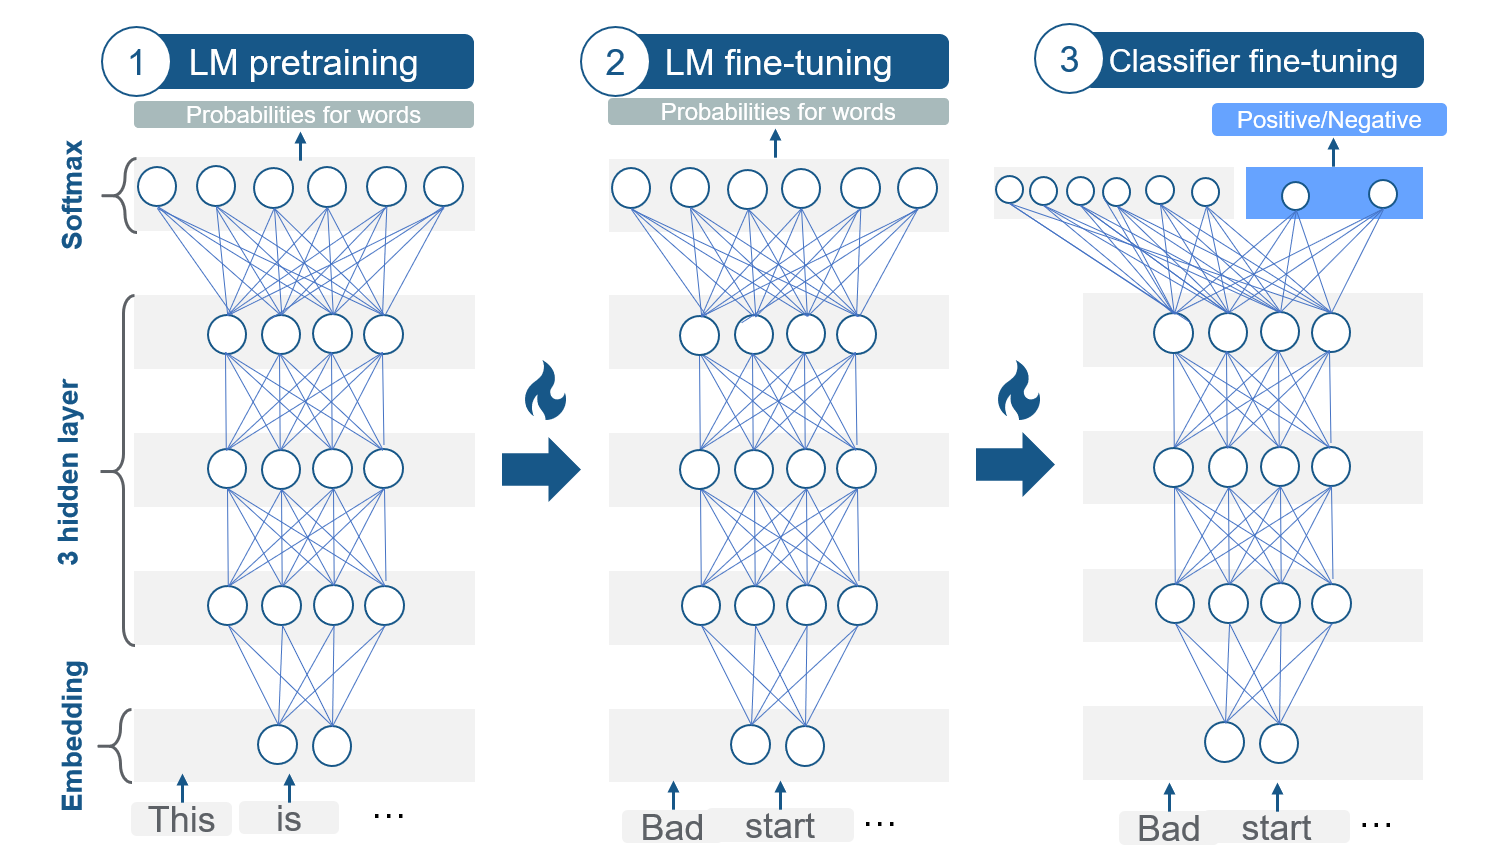
\includegraphics[width=0.9\textwidth]{ulmfit_process.png}
    \captionof{figure}{Quy trình 3 bước của ULMFiT: Pre-training trên dữ liệu chung, Fine-tuning LM trên dữ liệu miền đích, và Fine-tuning bộ phân loại cho tác vụ cuối cùng.}
    \label{fig:ulmfit_process}
\end{center}

\subsubsection{Các kỹ thuật Tinh chỉnh then chốt}
Sự thành công của ULMFiT không chỉ đến từ quy trình 3 bước mà còn từ 3 kỹ thuật tinh chỉnh thông minh được áp dụng trong bước cuối cùng.

\paragraph{1. Tinh chỉnh phân biệt (Discriminative Fine-tuning)}
Các tầng khác nhau của một mạng nơ-ron sâu nắm bắt các loại thông tin khác nhau: tầng đầu tiên học các đặc trưng rất chung chung, trong khi các tầng sau học các đặc trưng ngày càng cụ thể và phức tạp. Do đó, việc tinh chỉnh tất cả các tầng với cùng một tốc độ học (learning rate) là không hợp lý. ULMFiT đề xuất sử dụng các tốc độ học khác nhau cho mỗi tầng.

Giả sử mô hình có $L$ tầng, ta chọn một tốc độ học cơ sở $\eta_L$ cho tầng cuối cùng. Tốc độ học cho các tầng thấp hơn sẽ được tính bằng cách chia cho một hằng số (ví dụ: 2.6).
\[
\eta_{l-1} = \eta_l / \delta, \quad \text{với } \delta \text{ là một hằng số, ví dụ } 2.6.
\]
Khi cập nhật trọng số $\theta = \{\theta_1, \dots, \theta_L\}$, mỗi tầng sẽ được cập nhật như sau:
\begin{equation}
    \theta_l \leftarrow \theta_l - \eta_l \cdot \nabla_{\theta_l} J(\theta)
    \label{eq:discriminative_finetuning}
\end{equation}
Kỹ thuật này cho phép các tầng trên học hỏi nhanh chóng để thích nghi với tác vụ mới, trong khi các tầng dưới chỉ thay đổi một cách cẩn trọng để không làm mất đi kiến thức ngôn ngữ tổng quát đã học.

\paragraph{2. Tốc độ học Tam giác Lệch (Slanted Triangular Learning Rates - STLR)}
Thay vì giữ một tốc độ học không đổi hoặc giảm dần theo một hàm mũ đơn giản, ULMFiT sử dụng một lịch trình tốc độ học (learning rate schedule) đặc biệt. Trong một epoch, tốc độ học sẽ \textbf{tăng tuyến tính} trong một khoảng ngắn lúc đầu (warm-up), sau đó \textbf{giảm tuyến tính} trong phần còn lại của quá trình huấn luyện.

Công thức của STLR tại bước huấn luyện $t$ được định nghĩa như sau:
\begin{equation}
\eta_t = \eta_{\max} \times
\begin{cases}
    \frac{t}{t_{\text{cut}}} & \text{nếu } t < t_{\text{cut}} \\
    1 - \frac{t - t_{\text{cut}}}{T - t_{\text{cut}}} & \text{nếu } t \ge t_{\text{cut}}
\end{cases}
\label{eq:stlr}
\end{equation}
trong đó:
\begin{itemize}
    \item $T$ là tổng số bước huấn luyện trong một epoch.
    \item $t_{\text{cut}}$ là bước mà tại đó tốc độ học chuyển từ tăng sang giảm (thường là 10\% của $T$).
    \item $\eta_{\max}$ là tốc độ học tối đa, được chọn cho tầng cuối cùng. Các tầng khác sẽ có $\eta_{\max}$ riêng theo quy tắc của Tinh chỉnh phân biệt.
\end{itemize}
Chiến lược này giúp mô hình nhanh chóng hội tụ đến một vùng tham số tốt (giai đoạn tăng) rồi sau đó từ từ tinh chỉnh để tìm điểm tối ưu cục bộ tốt hơn (giai đoạn giảm).

\paragraph{3. Mở băng Dần dần (Gradual Unfreezing)}
Để tránh "sự quên lãng thảm khốc", việc tinh chỉnh toàn bộ mô hình ngay từ đầu trên một tập dữ liệu nhỏ có thể phá hỏng các trọng số đã được huấn luyện cẩn thận. ULMFiT đề xuất một phương pháp an toàn hơn, theo từng giai đoạn:

\begin{enumerate}
    \item \textbf{Giai đoạn 1:} Đóng băng (freeze) tất cả các tầng đã được huấn luyện trước ($l=1, \dots, L-1$), chỉ huấn luyện các tầng của đầu phân loại mới được thêm vào (tầng $L$) trong một epoch.
    \item \textbf{Giai đoạn 2:} Mở băng (unfreeze) tầng trên cùng của mô hình gốc (tầng $L-1$) và huấn luyện nó cùng với tầng $L$ trong một epoch nữa.
    \item \textbf{Giai đoạn 3 và tiếp theo:} Tiếp tục quá trình này, tuần tự mở băng từng tầng một từ trên xuống dưới ($L-2, L-3, \dots, 1$) và huấn luyện cho đến khi toàn bộ mô hình được tinh chỉnh.
\end{enumerate}
Phương pháp này giống như việc từ từ "rã đông" kiến thức, giúp mô hình thích nghi một cách nhẹ nhàng và hiệu quả, đặc biệt khi dữ liệu tác vụ có hạn.

\begin{tcolorbox}[
    title=Công thức thành công của ULMFiT,
    colback=green!5!white, colframe=green!50!black, fonttitle=\bfseries
]
ULMFiT không chỉ là một mô hình, mà là một công thức thực tiễn cho học chuyển giao trong NLP:
\begin{itemize}
    \item \textbf{Kiến trúc nền tảng:} AWD-LSTM (một biến thể LSTM hiệu quả và được điều chuẩn tốt).
    \item \textbf{Quy trình 3 bước:} Pre-train (chung) $\rightarrow$ Fine-tune LM (miền đích) $\rightarrow$ Fine-tune Classifier (tác vụ).
    \item \textbf{Bí quyết tinh chỉnh:} Kết hợp \textbf{Discriminative Fine-tuning}, \textbf{Slanted Triangular Learning Rates}, và \textbf{Gradual Unfreezing}.
\end{itemize}
\end{tcolorbox}

\subsubsection{Di sản và Hạn chế}
ULMFiT là một cột mốc quan trọng, nó đã "dân chủ hóa" việc áp dụng học chuyển giao trong NLP, cho thấy rằng không cần đến tài nguyên tính toán khổng lồ vẫn có thể đạt được hiệu suất cao. Nó đã đặt nền móng và tư duy cho các phương pháp sau này như BERT và các mô hình dựa trên Transformer, vốn cũng tuân theo quy trình "huấn luyện trước - tinh chỉnh" nhưng với kiến trúc mạnh mẽ hơn.

Tuy nhiên, hạn chế chính của ULMFiT nằm ở kiến trúc LSTM tuần tự, vốn không thể song song hóa hiệu quả và gặp khó khăn trong việc nắm bắt các phụ thuộc tầm xa so với kiến trúc Self-Attention của Transformer.

